% Label Quality Changes the Story — v3 (IAB @ NeurIPS 2026, Short Paper track)
%
% SUBMISSION REQUIREMENTS this file is built to satisfy (from
% https://iab-agents.github.io/ , Call for Papers → Submission Format):
%   * Short Paper: up to 4 PAGES + references + UNLIMITED APPENDIX
%   * NeurIPS-style formatting
%   * DOUBLE-BLIND review  → no author names, no affiliations, no identifying URLs
%   * Submission site: OpenReview
%   * Non-archival
%
% BEFORE SUBMITTING, three things still need you:
%   (1) the anonymized artifact URL in §5 (the real GitHub link is REMOVED — it
%       identifies the authors and would violate double-blind);
%   (2) the LLM-usage disclosure in Appendix C — only you can state this;
%   (3) verification of the three references, which were never checked.
\documentclass{article}

% Put the workshop's NeurIPS style file next to this .tex. The name below
% assumes `neurips_2026.sty`; if the organizers ship a different year, change
% this one line. Do NOT add the [final] option — that is camera-ready mode and
% it prints author names, breaking double-blind review.
\usepackage{neurips_2026}

\usepackage[utf8]{inputenc}
\usepackage[T1]{fontenc}
\usepackage{hyperref}
\usepackage{url}
\usepackage{booktabs}
\usepackage{amsmath}
\usepackage{amsfonts}
\usepackage{amssymb}
\usepackage{nicefrac}
\usepackage{microtype}
\usepackage{graphicx}
\usepackage{xcolor}

\title{Label Quality Changes the Story:\\What Actually Predicts a Coding Agent's Next Action}

% Double-blind: the NeurIPS style replaces this block with "Anonymous Author(s)"
% whenever the [final] option is absent. Leave it as-is for submission.
\author{%
  Anonymous Author(s) \\
  Affiliation \\
  Address \\
  \texttt{email} \\
}

\begin{document}

\maketitle

\begin{abstract}
Coding agents respond to every developer request through the same
undifferentiated pipeline, whether the request calls for implementing a feature,
diagnosing a bug, or searching a repository. We ask whether a developer's prompt
and recent session history can anticipate the agent's next \emph{action type}.
Using 8,404 real developer--agent turns mined from 251 GitHub repositories
containing SpecStory logs, we label the corpus three ways --- a rule, an LLM
judge, and human adjudication of a 212-turn sample --- and find that the two
automated labelings agree on only 42.5\% of turns ($\kappa=0.22$); against the
98 human-adjudicated turns the LLM label agrees far more often than the rule
(61.2\% vs.\ 31.6\%; $\kappa=0.512$ vs.\ $0.163$). Critically, the label changes
not just accuracy but \emph{the size of our headline finding}: under an
identical 5-fold repository-held-out protocol, the macro-F1 gain from adding
session history is $+45.6\%$ relative against the rule-based label and $+6.7\%$
against the LLM-assisted one. The smaller effect is consistent and statistically
supported (positive on all 5 folds; paired $t=10.40$, $p<0.001$), but an
ablation traces it almost entirely to one structured signal --- the previous
turn's action type --- and embedding the \emph{raw text} of prior turns performs
worse than using no history at all. Label construction is not a preprocessing
detail; it can determine what a study concludes.
\end{abstract}

\section{Introduction}

AI coding agents now sustain multi-turn collaborations spanning implementation,
debugging, explanation, review, and autonomous repository navigation --- yet
production systems typically route every request through the same model and tool
budget. A system that could anticipate a request's \emph{action type} before
generating a response could route \textsc{explain}-type requests to a cheaper
model, pre-warm a sandbox for anticipated \textsc{tool\_only} exploration, or
flag a \textsc{debug} request for a specialized workflow. Hence our question:
\emph{how well can a
developer's prompt and recent interaction history predict a coding agent's next
action, and what does that prediction actually depend on?} This is
query-difficulty routing [Ong et al., 2025] applied to action type rather than
difficulty; our results suggest an action-aware router would need session-level
features, not a single-turn query encoder alone. Two contemporaneous studies
mine the same SpecStory-log source, building a taxonomy of collaboration
patterns [Tang et al., 2026] and linking chat behavior to contribution outcomes
[Fang et al., 2026]; both validate the source at scale, but neither asks a
forward-looking, per-turn prediction question.

Studying this on real transcripts rather than synthetic data forces us to
confront a problem central to this workshop's scope: constructing behavioral
labels for agent runs is itself unreliable, and that unreliability does not
merely add noise --- it can change which claims a study supports. We report
three findings we believe are useful beyond our dataset: (1) two defensible
labelings of the same turns agree on less than half of them, and against human
adjudication the LLM-assisted label agrees roughly twice as often as the rule;
(2) the size of a central empirical claim shrinks nearly sevenfold once the
label changes, though it stays consistent and statistically supported; and (3)
\emph{how} context is represented matters more than \emph{how much} of it there
is.

\section{Data and Labeling}

\textbf{Corpus.} We mine SpecStory session logs --- Markdown transcripts that
Cursor/Copilot-style tools write to \texttt{.specstory/history/}, capturing full
developer--agent turns (prompts, responses, generated code, tool calls) --- from
public GitHub repositories that committed them, discovered via six GitHub Search
API queries. From 68,943 extracted turn pairs, after noise filtering, a
stratified per-repository cap (preserving each repository's action-type mix),
and machine translation of the 31\% of prompts not originally in English, we
obtain \textbf{8,404 turns across 251 repositories} and 3,191 session logs. The
corpus is not repository-dominated (Gini 0.299; top 10 supply 5.9\% of turns).

\textbf{A parsing failure worth naming.} An earlier parser bug left blank
\texttt{agent\_response} values in \textbf{48.4\%} of raw turn pairs, falling to
\textbf{29.8\%} once fixed; those extra blanks were routed into low-information
categories, inflating the apparent value of history. All results below use the
corrected extraction; Appendix~\ref{app:parser} gives the failure mode and how
we caught it.

\textbf{Three-tier labeling.} \texttt{action\_type} does not exist in the raw
data. \emph{Tier 1} is a deterministic rule using tool-use flags,
generated-code volume, and prompt-side keyword regexes. \emph{Tier 2} is an LLM
(Gemini) prompted with our category definitions, the full prompt and response
text, and the same metadata, returning a label with a rationale. \emph{Tier 3}
is human adjudication of a 212-turn sample drawn by stratifying on the
\emph{LLM's} predicted class, up to 40 turns per class (\textsc{implement} 40,
\textsc{explain} 40, \textsc{other} 40, \textsc{tool\_only} 40, \textsc{debug}
39, \textsc{review} 13 --- the last two classes had smaller pools). The sample
was \emph{not} drawn from disagreements; 98 of the 212 happened to be turns
where the rule and the LLM disagreed, and those 98 were adjudicated by one
author.

The two automated labelings agree on only \textbf{42.5\%} of the corpus
($\kappa = 0.223$), and the disagreement is structural rather than diffuse:
1,448 turns the rule calls \textsc{implement} the LLM calls \textsc{debug}, and
646 turns the rule calls \textsc{tool\_only} the LLM calls \textsc{implement}.
\textsc{debug} is 3.5\% of the corpus under the rule and 26.6\% under the LLM;
\textsc{tool\_only} falls from 16.9\% to 5.8\%. Inspecting disagreements shows
why: the rule flags \textsc{tool\_only} whenever no literal code fence appears,
but many turns make real edits through tool calls with no inline code block ---
the rule's blind spot, not a behavioral difference.

\begin{table}[t]
\caption{Agreement with human judgment on the 98 adjudicated turns (no
imputation: every cell is scored against a real human label). ``LLM (initial)''
is the labeling the adjudicator saw; ``LLM (refined)'' is the relabeling used
for every experiment in Section~\ref{sec:results}.}
\label{tab:agreement}
\centering
\small
\begin{tabular}{lrccc}
\toprule
Human label & $n$ & Rule & LLM (initial) & LLM (refined) \\
\midrule
\textsc{implement} & 13 & 0.08 & 0.69 & 0.69 \\
\textsc{debug}     & 30 & 0.60 & 0.33 & \textbf{0.83} \\
\textsc{explain}   & 15 & 0.20 & \textbf{0.80} & 0.53 \\
\textsc{review}    & 16 & 0.38 & 0.44 & 0.38 \\
\textsc{tool\_only}& 12 & 0.25 & \textbf{0.58} & 0.08 \\
\textsc{other}     & 12 & 0.00 & 0.92 & 0.92 \\
\midrule
Overall accuracy & 98 & 0.316 & 0.571 & \textbf{0.612} \\
Cohen's $\kappa$ & 98 & 0.163 & 0.482 & \textbf{0.512} \\
\bottomrule
\end{tabular}
\end{table}

\textbf{What adjudication does and does not establish.} The LLM label agrees
with the human roughly twice as often as the rule ($\kappa = 0.482$ vs.\
$0.163$; Table~\ref{tab:agreement}). Adjudication also exposed two definitions
doing no work, so we sharpened them --- \textsc{debug} around \emph{a concrete
root cause was identified} rather than \emph{a stack trace was present},
\textsc{review} around \emph{no reported problem is driving this} --- and
relabeled. That raised agreement to $\kappa = 0.512$, but not uniformly:
\textsc{debug} rose from 0.33 to 0.83 while \textsc{explain} fell from 0.80 to
0.53 and \textsc{tool\_only} collapsed from 0.58 to 0.08. We therefore adopt the
refined label as a \emph{working} label, not ground truth: it is the labeling
that best agrees with a careful human reader, and that reader still disagrees
with it on roughly four turns in ten. Two limits: the $\kappa$ values come from
turns selected as rule/LLM disagreements, which are harder than average, and the
adjudicator saw the initial LLM label.

\section{Modeling and Results}
\label{sec:results}

We compare representations of increasing richness --- TF-IDF,
sentence-embedding (\texttt{all-MiniLM-L6-v2}) prompt-only, $+$ prompt surface
features, $+$ leakage-safe prior-turn history (previous action type, whether
that turn had code/tools, rolling session code-rate, turn position --- all
\texttt{shift(1)}'d so nothing from the current turn leaks in), and the full
combination --- each with four model families (logistic regression, random
forest, MLP, XGBoost). Repositories, not rows, are split 80/20
(\texttt{GroupShuffleSplit}: 200/51 repositories, 6,665/1,733 turns, zero
overlap), and we additionally run 5-fold repository-held-out
\texttt{GroupKFold}, reusing the same folds across representations so per-fold
scores are paired. Holding repositories out is an evaluation-design choice ---
it stops a model scoring well by memorizing project vocabulary --- not a
measurement of cross-repository generalization, which we do not attempt.
Baselines: majority-class, and a prompt-only keyword rule. Full results appear
in Appendix~\ref{app:results}.

\textbf{Prediction is possible but modest.} Against the refined label, the
prompt alone reaches macro-F1 $0.341 \pm 0.014$ over six classes --- well above
the majority-class baseline (0.086) but only modestly above a hand-written
keyword rule over the same text (0.320, single split). Per-class F1 is highly
uneven (\textsc{debug} 0.72, \textsc{implement} 0.62, \textsc{explain} 0.41,
\textsc{review} 0.26, \textsc{other} 0.23, \textsc{tool\_only} 0.04): the
classes the model predicts are those the labelers agree on, and
\textsc{tool\_only} --- where the refinement most damaged human agreement
(Table~\ref{tab:agreement}) --- is also the one it cannot predict at all. The
headline number aggregates a task that is learnable for two classes and close to
unlearnable for two others, not uniform six-way competence.

\textbf{Adding history helps, consistently but slightly.} Prior-turn features
raise macro-F1 to $0.364 \pm 0.017$. The improvement is positive on every one of
the 5 paired folds ($+0.030, +0.018, +0.027, +0.021, +0.020$; paired
$t = 10.40$, $p = 0.00048$; Wilcoxon $p = 0.0625$, which is the smallest value
attainable at $n{=}5$ and is reached precisely because all folds agree in sign).
The direction also holds for MLP and XGBoost under the same protocol; random
forest is the exception, essentially flat at $0.215 \to 0.216$
(Appendix~\ref{app:results}, Table~\ref{tab:cvfull}). The effect is real and
reproducible. It is also small enough that we would not expect a routing
decision to change because of it.

\begin{figure}[t]
\centering
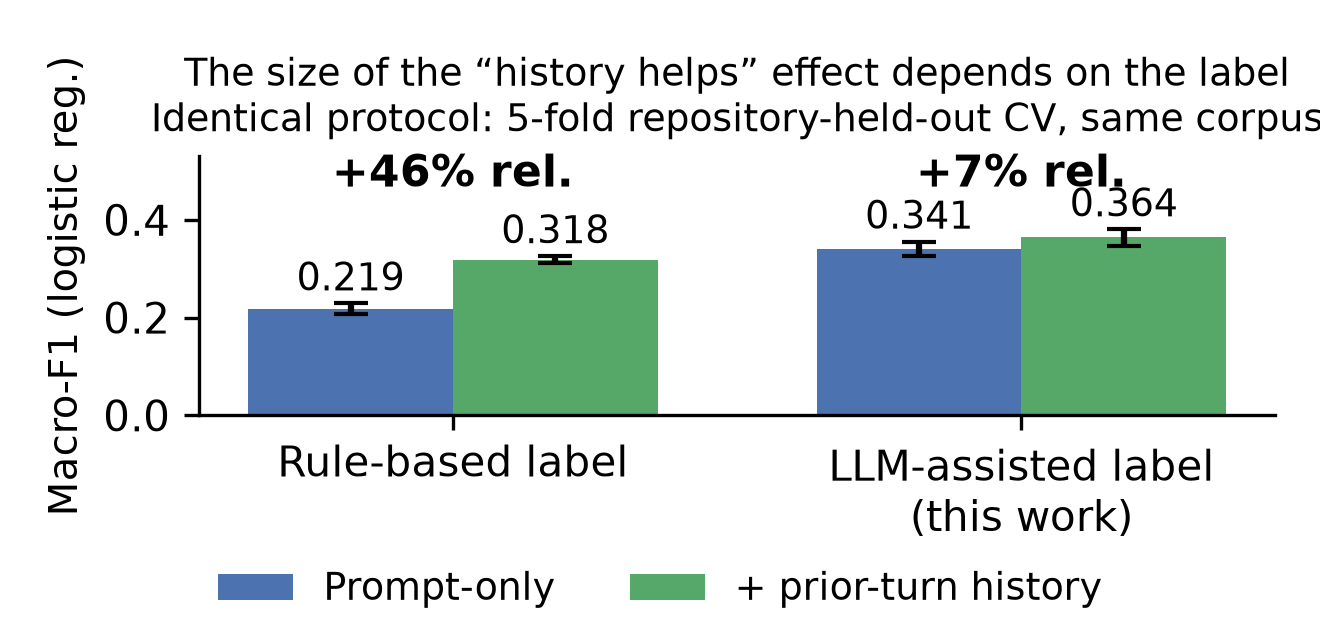
\includegraphics[width=0.68\textwidth]{figures/fig2_label_quality_effect.png}
\caption{The same experiment run against two label sources under an identical
protocol (5-fold repository-held-out CV, logistic regression, same corpus). The
rule-based label overstates the relative effect of adding session history by
roughly sevenfold.}
\label{fig:labelquality}
\end{figure}

\textbf{Label quality changes the size of the finding, not just its level.}
Figure~\ref{fig:labelquality} makes this explicit. Measured against the
rule-based label, the same prompt-only-vs.-history comparison shows a
$\mathbf{+45.6\%}$ relative macro-F1 gain ($0.219 \to 0.318$); measured against
the refined LLM label it is $\mathbf{+6.7\%}$ ($0.341 \to 0.364$). Both come
from the same modeling pipeline, the same corpus, the same folds, and the same
model --- only the label changed. This is an observational comparison of two
labeling pipelines, not a randomized manipulation, so we claim the measured
effect size differs sharply by label, not that label noise \emph{causes} a
specific inflation. The plausible account is that the rule's label is partly a
function of response-side surface features that persist across adjacent turns,
making the previous turn's label unusually predictive of the current one.

\textbf{Ablation: one feature accounts for the measured gain.} Isolating
\emph{previous action type} alone (dropping code/tool/turn-position features)
reaches $0.361 \pm 0.018$ against the full bundle's $0.364$. A paired test over
the same folds finds no detectable difference (paired $t = -2.12$, $p = 0.102$;
Wilcoxon $p = 0.1875$) --- an absence of evidence at $n{=}5$, not evidence of
equivalence. What it supports is narrow but useful: the other session-state
features we engineered add nothing measurable on top of knowing what the agent
did last turn.

\textbf{Negative result: raw-text context underperforms.} Concatenating the
actual text of the previous $N=1,2,3$ turns and re-embedding it, instead of
using structured summary features, underperforms the plain prompt-only embedding
at every $N$ (best: $N{=}1$, macro-F1 0.303 vs.\ 0.341, single split). This is a
result about representation, not information: what happened last turn is
available to our models as a category but \emph{not} recoverable from the raw
words, plausibly because concatenation dilutes the current prompt's embedding.
It does not establish that prior-turn text carries no lexical signal --- a
longer-context or fine-tuned encoder might extract it. Repository metadata
(language, stars, size, age) was a second plausible context source that did not
help ($0.362$ vs.\ $0.364$).

\section{Threats to Validity}

Four limits bear directly on the numbers above; Appendix~\ref{app:threats} gives
the full account. \emph{Label validation is thin}: adjudication is
single-annotator over 98 turns, not blind to the LLM's label, and those turns
were selected as rule/LLM disagreements rather than at random, so
Table~\ref{tab:agreement} is an estimate on hard cases. \emph{The taxonomy was
revised mid-study}, which tempers any claim to objective ground truth --- though
the initial-LLM $\kappa$ was computed \emph{before} that revision, so that
estimate is not circular. \emph{Statistical power is low}: paired tests use 5
folds and one model family, and the rule-label condition has no paired test of
its own. \emph{Selection is narrow}: the corpus covers only developers who used
SpecStory \emph{and} committed the logs publicly, skewing toward experimental or
process-transparent practice.

\section{Conclusion}

Anticipating a coding agent's next action from session context is possible but
modest, and the reported \emph{size} of that possibility depends heavily on how
the behavioral label was constructed. Two defensible labelings of the same 8,404
turns agree on less than half of them and disagree by an order of magnitude
about how much of coding-agent work is debugging; run through an identical
pipeline, they report a history effect of $+46\%$ and $+7\%$. An ablation then
shows a single structured feature accounts for what remains. For anyone building
automated behavior labels for agent trajectories, checking the label against
independent human judgment is not optional diligence --- it can change what the
resulting study is a study \emph{of}.

% ANONYMITY: the public GitHub link was REMOVED — it names an author and this
% venue is double-blind. Replace the red placeholder below with an anonymized
% mirror (e.g. anonymous.4open.science) before submitting. Keep it to one line.
\paragraph{Artifacts.} The corpus, all three label sets, the human review sheet,
every results table (including per-fold CV and paired significance tests), and
the full pipeline are released at \textcolor{red}{[ANONYMIZED URL]}.

\section*{References}
\small

Zihan Fang, Yueke Zhang, Ningzhi Tang, Collin McMillan, Toby Jia-Jun Li, and Yu
Huang. From conversation to contribution: Characterizing vibe coding in
open-source software. \emph{arXiv preprint arXiv:2607.05677}, 2026.

Isaac Ong, Amjad Almahairi, Vincent Wu, Wei-Lin Chiang, Tianhao Wu, Joseph E.
Gonzalez, M. Waleed Kadous, and Ion Stoica. RouteLLM: Learning to route LLMs
with preference data. In \emph{International Conference on Learning
Representations (ICLR)}, 2025.

Ningzhi Tang, Chaoran Chen, Zihan Fang, Gelei Xu, Maria Dhakal, Yiyu Shi, Collin
McMillan, Yu Huang, and Toby Jia-Jun Li. Programming by chat: A large-scale
behavioral analysis of 11,579 real-world AI-assisted IDE sessions. \emph{arXiv
preprint arXiv:2604.00436}, 2026.

\normalsize
\newpage
\appendix

\section{Full Results}
\label{app:results}

\begin{figure}[h]
\centering
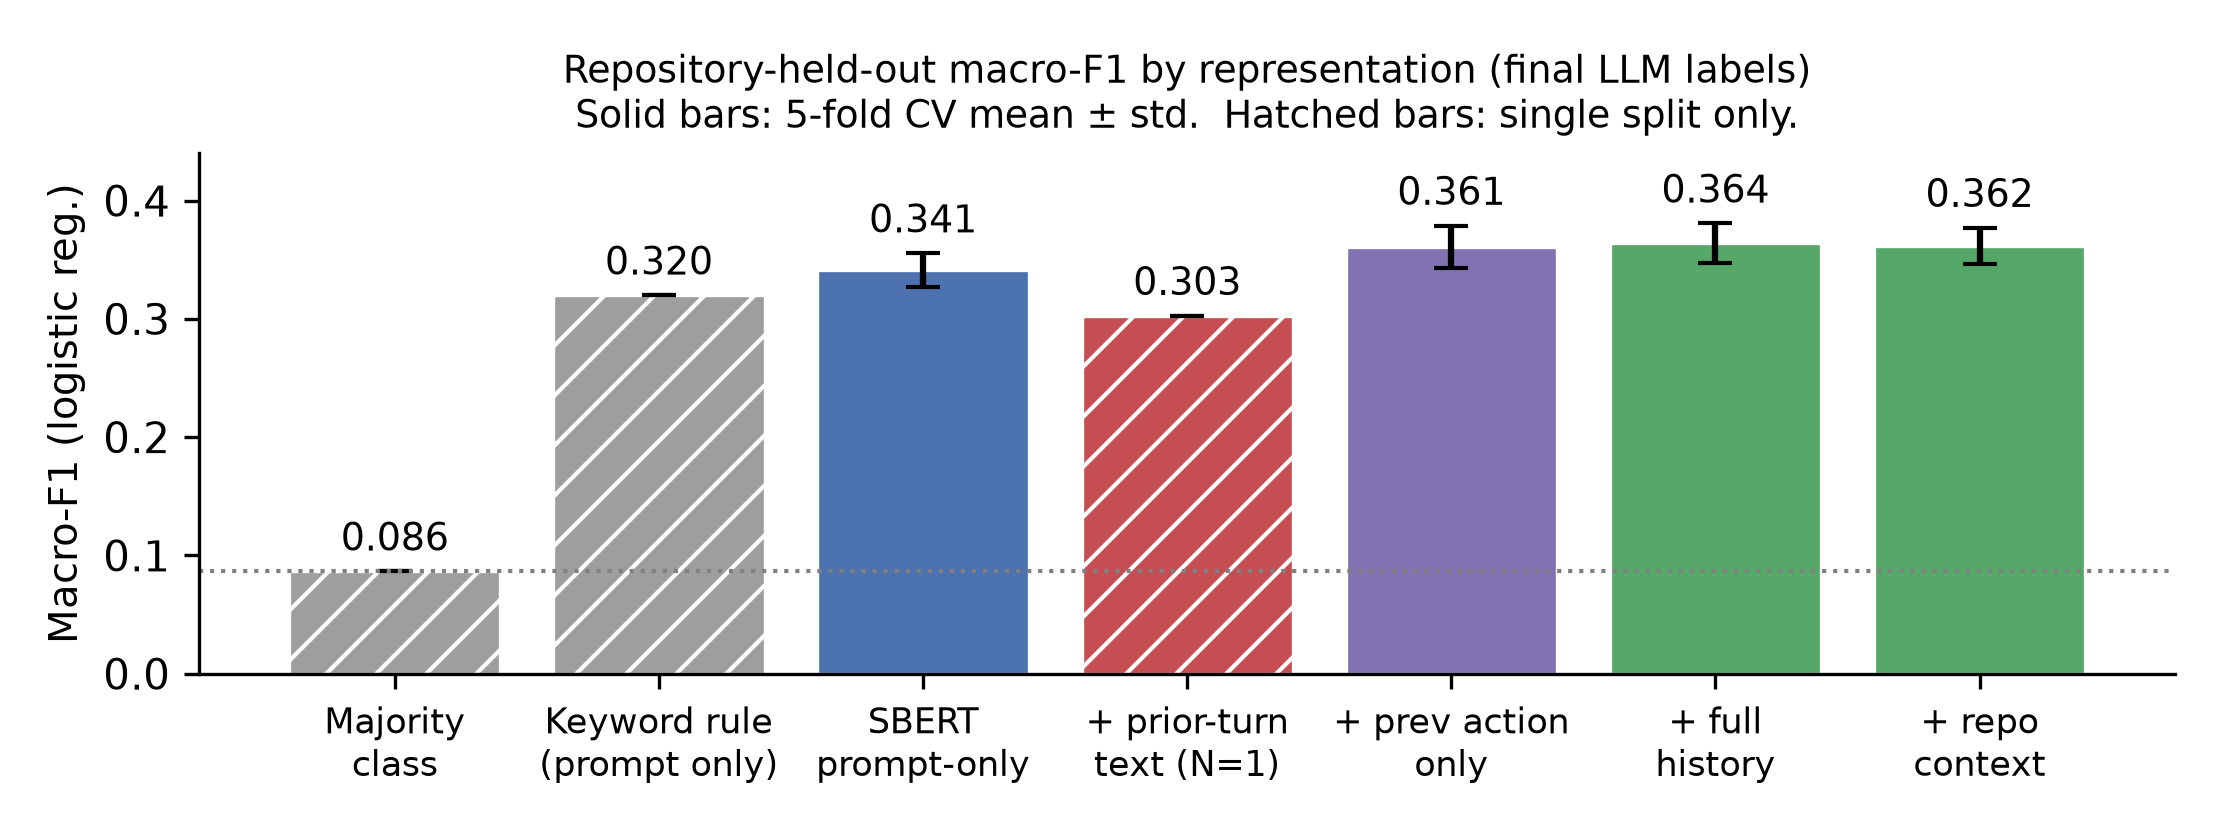
\includegraphics[width=0.92\textwidth]{figures/fig1_headline_macrof1.png}
\caption{Macro-F1 by representation under the refined LLM label. Solid bars are
5-fold repository-held-out CV (mean $\pm$ std); hatched bars are available only
from the single split. The two protocols are marked rather than mixed.}
\label{fig:headline}
\end{figure}

\begin{table}[h]
\caption{5-fold repository-held-out CV macro-F1 (mean $\pm$ std) under the
refined LLM label, all representations $\times$ model families.}
\label{tab:cvfull}
\centering
\small
\begin{tabular}{lcccc}
\toprule
Representation & Logistic reg. & MLP & XGBoost & Random forest \\
\midrule
SBERT prompt-only              & $0.341 \pm 0.014$ & $0.338 \pm 0.021$ & $0.288 \pm 0.010$ & $0.215 \pm 0.006$ \\
$+$ prev.\ action only         & $0.361 \pm 0.018$ & $0.349 \pm 0.015$ & $0.298 \pm 0.010$ & $0.224 \pm 0.006$ \\
$+$ history                    & $0.364 \pm 0.018$ & $0.361 \pm 0.025$ & $0.312 \pm 0.007$ & $0.221 \pm 0.007$ \\
$+$ metadata $+$ history       & $0.364 \pm 0.017$ & $0.364 \pm 0.024$ & $0.308 \pm 0.009$ & $0.215 \pm 0.007$ \\
$+$ repo context               & $0.362 \pm 0.015$ & $0.348 \pm 0.022$ & $0.322 \pm 0.017$ & $0.213 \pm 0.007$ \\
\bottomrule
\end{tabular}
\end{table}

\begin{table}[h]
\caption{Paired tests on the 5 repository-held-out folds (logistic regression;
the same folds are reused across representations, so per-fold scores are
paired). At $n{=}5$ the smallest attainable Wilcoxon $p$-value is $0.0625$.}
\label{tab:paired}
\centering
\small
\begin{tabular}{lccc}
\toprule
Comparison & Mean $\Delta$ & Paired $t$ ($p$) & Wilcoxon $p$ \\
\midrule
prompt-only $\to$ $+$metadata$+$history & $+0.0229$ & $10.40$ ($0.00048$) & $0.0625$ \\
$+$metadata$+$history $\to$ prev.\ action only & $-0.0029$ & $-2.12$ ($0.102$) & $0.1875$ \\
\bottomrule
\end{tabular}
\end{table}

Fold-wise differences for the first comparison are
$+0.0296, +0.0178, +0.0265, +0.0207, +0.0200$ --- positive on every fold. For
the second they are $-0.0044, -0.0010, -0.0037, -0.0067, +0.0013$, mixed in
sign.

\section{The Parser Failure in Detail}
\label{app:parser}

SpecStory sometimes represents one logical agent turn as several consecutive
Markdown blocks (one per tool call, plus prose). An earlier version of our
parser read only the first block and discarded the rest, including the turn's
closing content, and reduced a pure tool-call block to an empty string rather
than to a marker that something had happened. The rule labeler then routed those
blank responses into \textsc{other}/\textsc{review} by default, which made the
affected rows trivially predictable once the previous (equally affected) turn's
label was known --- inflating the apparent value of session history.

The bug was not caught by a test. It was caught by asking why an early
inter-labeler agreement check was anomalously near zero for exactly two classes
(\textsc{tool\_only} and \textsc{review}), sampling one disagreement, and reading
the raw transcript, where a turn flagged as using tools had an empty response.

We report this because the failure mode is intrinsic to trajectory mining:
transcript formats are undocumented, heterogeneous, and evolving, and a parser
that silently drops content yields a corpus that looks fine, trains fine, and
reports a stronger effect than the truth. A class-level agreement breakdown
between two independent labelers proved to be a cheap and unusually effective
canary for it.

\section{Threats to Validity in Full}
\label{app:threats}

\textbf{Label validation is thin.} Adjudication is single-annotator over 98
turns, not blind to the LLM's label, and those turns were selected as rule/LLM
disagreements rather than at random. \textsc{review} contributes only 13 turns
to the sampling pool and 16 human labels, so its per-class numbers in
Table~\ref{tab:agreement} should be read as indicative only. A fresh 240-turn
sample drawn from the refined label set is released unadjudicated; adjudicating
it is the obvious next step. Our taxonomy was also revised mid-study based on
this pass, which tempers any claim to an objective ground truth --- though the
$\kappa$ values for the initial LLM labeling were computed \emph{before} that
revision, so that particular estimate is not circular.

\textbf{Statistical scope.} Paired tests use 5 folds and one model family; power
is correspondingly low, and we report $p$-values plainly rather than as evidence
of a large effect. The rule-label condition in Figure~\ref{fig:labelquality} has
CV means and standard deviations but no paired test of its own.

\textbf{Corpus and representation.} Our corpus covers only repositories where a
developer both used SpecStory \emph{and} committed the logs publicly --- almost
certainly skewed toward experimental or process-transparent developers, though
two contemporaneous studies mining the same source [Tang et al., 2026, Fang et
al., 2026] report comparable corpus sizes, suggesting this is a property of the
data source rather than our query design. The per-repository cap samples turns,
so a turn's immediate predecessor may not survive into the corpus even though
its history features were computed from the complete session; this disadvantages
the raw-text experiment. Finally, all results use one sentence-embedding model;
we do not know whether a code-aware or longer-context encoder would change the
size --- or, for raw text, possibly the direction --- of these effects.

\section{Ethics, Data, and LLM Usage}
\label{app:ethics}

\textbf{Data provenance.} All transcripts analyzed here were already public:
they are files that developers chose to commit to public GitHub repositories,
retrieved through the GitHub Search and Contents APIs under GitHub's terms of
service. No private repositories, credentials, or non-public data were accessed.
No human participants were recruited, no interaction was solicited, and no
demographic attributes were collected or inferred, so the work did not involve
human-subjects research; the only human annotation is adjudication performed by
an author on the authors' own dataset.

\textbf{Residual privacy risk.} Developer prompts are natural-language text and
can incidentally contain identifying detail (names, project paths, occasionally
pasted configuration). We report only aggregates and short illustrative
fragments, and the released artifacts preserve the repository identifiers needed
for reproduction. Readers who reuse this corpus should treat it as
personally-identifiable-adjacent text rather than as anonymized data.

\textbf{LLM usage.} An LLM (Gemini) is used as a research instrument in this
work: it produces the Tier-2 \texttt{action\_type} labels described in Section 2.
Its role, prompt design, category definitions, and measured agreement with human
judgment are reported in the body of the paper rather than treated as a black
box, and both the labels and the label-generating code are released.
\textcolor{red}{[AUTHORS: the venue requires adherence to the NeurIPS 2026
policies on the use of agents and large language models. State here, accurately,
any use of LLMs in \emph{writing or preparing} this manuscript, as distinct from
the labeling use described above. Do not leave this bracket in the submitted
PDF.]}

\end{document}
